\documentclass[twoside,11pt]{article}

% Additional packages
\usepackage{jmlr2e}
\usepackage{amsmath}
\usepackage{graphicx}
\usepackage{natbib} % For citations
\usepackage{hyperref}
\usepackage{setspace}
\usepackage{float}
\usepackage{placeins}


% Handy macros
\newcommand{\dataset}{{\cal D}}
\newcommand{\fracpartial}[2]{\frac{\partial #1}{\partial  #2}}


\jmlrheading{1}{2024}{1-5}{10/12}{10/12}{Valentine Dumange, Ying Tong Chen, Danial Shafaei}

\ShortHeadings{Image Deblurring Using Adaptive Kernel Estimation}{Dumange, Chen, Shafaei}
\firstpageno{1}


\begin{document}

\title{Image Deblurring Using Adaptive Kernel Estimation and Wiener Deconvolution}

\author{\name Valentine Dumange \email valentine.dumange@tprs.stud.vu.lt \\
\AND
    \name Ying Tong Chen \email chen.ying-tong@tprs.stud.vu.lt\\
\AND
    \name Danial Shafaei \email danial.shafaei@mif.stud.vu.lt \\\\
       \addr Data Science Study Programme\\
       Faculty of Mathematics and Informatics}

\editor{Jurgita Markevi\v{c}i\={u}t\.{e}}

\maketitle

\begin{abstract}
With smartphones now widely accessible, capturing moments through photography has become effortless. However, various factors often degrade image quality, causing blurring and noise. For instance, Gaussian blur due to the defocus of a camera, motion blur from hand tremors, further reduce clarity. This study aims to utilize a machine learning regression model to predict blur kernels (Point Spread Functions, PSFs) corresponding to specific image features and apply Wiener deconvolution to restore image details.
\end{abstract}

\begin{keywords}
  Image Deblurring, Adaptive Kernel Estimation, Wiener Deconvolution, Machine Learning, Noise Reduction
\end{keywords}

\section{Introduction}
Image blur is a persistent challenge in digital photography that significantly impacts image quality and visual information retention. The problem of image restoration has been a central focus in signal processing since the advent of digital imaging, with groundbreaking work by \citet{molina2001image} establishing Bayesian frameworks for astronomical image restoration. Early restoration techniques, as comprehensively reviewed by \citet{banham1997digital}, were primarily developed for space exploration, medical imaging applications, and astronomical observations. These applications demanded highly specialized deblurring approaches due to their unique imaging conditions and quality requirements. As digital photography evolved from its inception in the 1970s through Kodak's first digital camera prototype, to today's ubiquitous smartphone cameras, the challenge of blur has remained constant, though its sources have varied and become more complex. This degradation can occur through various mechanisms, including camera motion, defocus, or atmospheric turbulence, each presenting unique challenges for restoration algorithms. While numerous deblurring techniques exist, most either require precise knowledge of the blur kernel or rely on computationally intensive deep learning approaches that may not be practical in all scenarios, particularly in resource-constrained environments or real-time applications.
\singlespacing
Traditional deblurring methods often assume a uniform blur kernel across the entire image, a simplification first challenged by \citet{cannon1976blind} in their seminal work on blind deconvolution. Their research demonstrated that phase information in the frequency domain could be utilized for blur identification, laying the groundwork for modern blind deconvolution techniques. This uniform kernel assumption fails to account for spatially varying blur patterns commonly found in real-world photographs, where different regions of an image may experience different types and degrees of blur. While \citet{fish1995blind} made significant advances with their Richardson-Lucy algorithm approach to spatially-varying kernels in the 1990s, demonstrating impressive reconstruction quality with only 1.0\% error in point-spread function evaluation, the computational constraints of the era limited practical applications. Their work showed particular promise in handling noise-corrupted images, outperforming contemporary blind deconvolution methods. Today, existing adaptive methods typically require significant computational resources or extensive training data, limiting their practical applications, especially in mobile devices or embedded systems where processing power and memory are constrained. This creates a pressing need for more efficient, adaptive approaches that can maintain high restoration quality while reducing computational overhead.
\singlespacing
This study aims to:
\begin{itemize}
\item Develop a machine learning-based approach for adaptive kernel estimation that can handle various blur types
\item Create an efficient method for predicting appropriate blur kernels based on local image characteristics
\item Implement and validate a combined system using predicted kernels with Wiener deconvolution
\item Evaluate the performance across different blur scenarios and noise conditions
\end{itemize}
\singlespacing
The proposed approach bridges the gap between computationally intensive deep learning methods and traditional fixed-kernel approaches. By developing a machine learning model that can predict appropriate blur kernels based on image features, we aim to achieve better deblurring results while maintaining reasonable computational requirements. This research has practical applications in:
\begin{itemize}
\item Mobile photography enhancement
\item Medical image processing
\item Surveillance system improvement
\item Historical photo restoration
\end{itemize}
\singlespacing
Our approach combines traditional image processing techniques with modern machine learning methods. We first extract relevant features from blurred images, use these features to predict appropriate blur kernels through a regression model, and then apply Wiener deconvolution using the predicted kernels. This methodology allows for adaptive kernel selection while maintaining computational efficiency.

\section{Literature Review}

\subsection{Introduction to Image Degradation Model}
The mathematical model for image degradation is typically represented as:
\[
g(x, y) = h(x, y) * f(x, y) + n(x, y)
\]
where \( g(x, y) \) represents the degraded image, \( h(x, y) \) is the point spread function (PSF), \( f(x, y) \) is the original image, and \( n(x, y) \) is the added noise. This model underlies both non-blind and blind image deblurring methods, serving as the foundation for kernel estimation and image reconstruction processes.

\subsection{Traditional Image Deblurring Methods}
Traditional image deblurring methods generally consist of two steps: estimating the blur kernel (PSF) and reconstructing the image. This approach, known as non-blind image deblurring, involves restoring the observed blurred image \( g(x, y) \) using the estimated blur kernel \( h(x, y) \) to approximate the clear image \( f'(x, y) \). Because multiple methods are available for estimating blur kernels, non-blind deblurring is often considered an ill-posed problem.

Early non-blind deblurring methods include Inverse Filtering \citep{saberi1999inverse}, Wiener filtering \citep{wiener1949extrapolation}, and Richardson-Lucy deconvolution \citep{richardson1972bayesian}. These techniques rely on an accurately known blur kernel to perform deblurring, making kernel estimation a necessary prerequisite.

\subsection{Frequency Domain Approaches for PSF Estimation}
In the frequency domain, the Fourier Transform (FFT) of a blurred image can assist in estimating the PSF. Different types of blur exhibit distinct frequency patterns; for instance, motion blur often appears as directional lines in the frequency spectrum, while Gaussian blur displays a radially symmetric pattern \citep{john2020fourier}. Analyzing these frequency patterns provides an initial estimate of the blur kernel, which can then be refined iteratively.

Further methods, such as inverse filtering in the frequency domain, require estimating the blur kernel and the signal-to-noise ratio (SNR). Iterative estimation techniques can refine the PSF by adjusting it to better match the frequency characteristics of the image, commonly applied in blind deblurring.

\subsection{Non-Blind Image Deblurring Using Deep Learning}
Recently, deep learning techniques have been applied to non-blind deblurring tasks. For example, \citet{dong2024dwdn} employed deep learning to model the PSF, which is then combined with Wiener filtering to restore the image. These methods leverage deep learning’s ability to capture complex patterns, but they often require large datasets and extensive computational resources.

\subsection{Blind Image Deblurring Techniques using Deep Learning}
Blind image deblurring techniques do not require prior knowledge of the blur kernel (or PSF) and aim to estimate the kernel while recovering the original image. Deep learning models, such as the CNN-based approach by \citet{nah2016multi} and the DeblurGAN model \citep{kupyn2018deblurgan}, are capable of removing blur without explicitly estimating a blur kernel. These techniques can handle various blur types effectively, offering promising results in image deblurring tasks \citep{amrollahi2023survey}.

\subsection{Machine Learning for Kernel Prediction and Noise Classification}
Traditional machine learning techniques offer advantages in interpretability, smaller model size, and lack of reliance on large datasets, making them suitable for specific applications. These techniques can also aid in noise classification, allowing the development of distinct blur kernel prediction models for different blur types, such as Gaussian and motion blur. This targeted approach offers flexibility for situations where deep learning is not feasible.

\subsection{Conclusion and Proposed Approach}
While deep learning methods achieve high performance in image deblurring tasks, they often require large datasets and considerable computational resources. This project proposes a machine learning-based model that dynamically selects blur kernels based on specific image features, integrating traditional deblurring techniques with machine learning adaptability. By employing Wiener deconvolution, this approach aims to improve image clarity and reduce blur artifacts effectively across diverse scenarios.


\section{Data}

\subsection{Dataset}
We chose the DIV2K (DIVerse 2K Resolution Dataset) as our training dataset. Although it is widely used for image super-resolution tasks, its high quality and diverse content make it an excellent choice for our image deblurring project. DIV2K consists of 1,000 high-resolution images (typically 2048×1080 or 2048×2048) featuring various scenes such as natural landscapes, buildings, animals, and people. The dataset’s rich variety of textures and structures helps ensure robust model performance across different scenarios.

\subsection{Data Preprocessing}
To enhance training efficiency, we randomly cropped the original images into 256×256 patches. However, we observed that some images were already blurred due to camera focal length issues. To address this, we manually removed such images before applying blur kernels.

\begin{figure}[H]
\centering
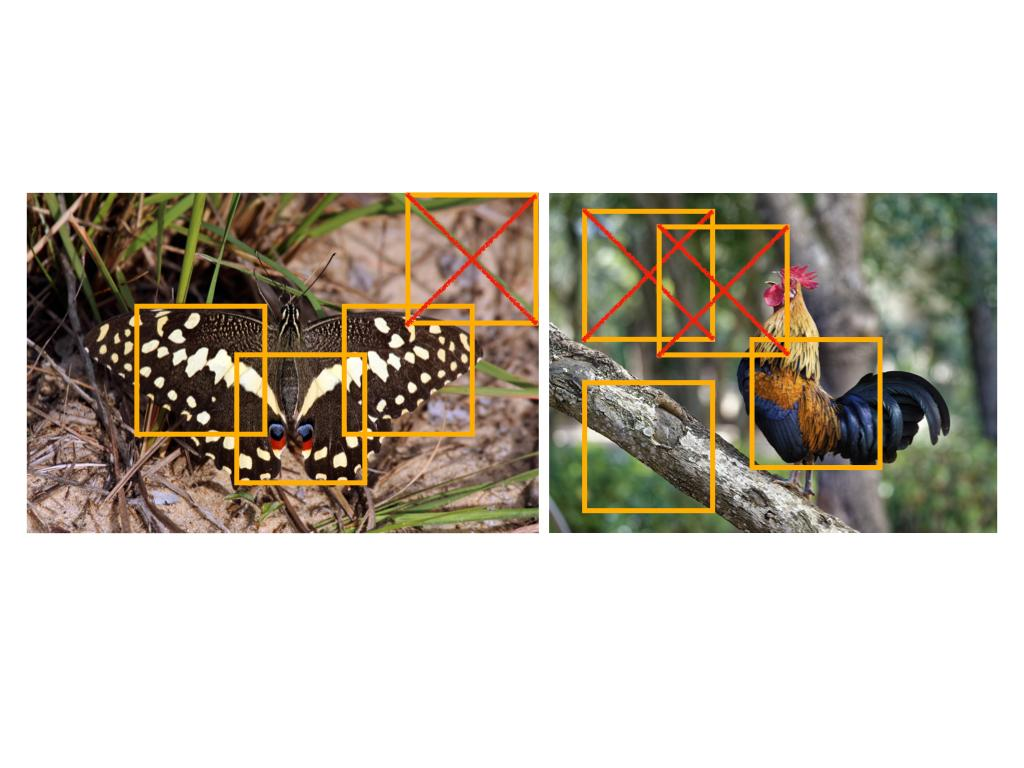
\includegraphics[width=0.7\textwidth]{figure1.jpg}
\caption{Illustration of the training dataset. Some images focus only on objects in the foreground, which may result in nearly blurred patches during random cropping. To address this, we manually remove such cases. Additionally, images with large areas of uniform color are also filtered out beforehand.}
\end{figure}

\subsection{Feature Extraction}

\subsubsection{Sobel}
The Sobel operator is a widely used edge-detection technique in image processing and computer vision. It computes the gradient magnitude of an image by applying two convolutional kernels, one for detecting horizontal changes (\(x\)-direction) and another for vertical changes (\(y\)-direction). These kernels emphasize regions with high spatial frequency, such as edges. The Sobel operator is computationally efficient and robust to noise, making it ideal for identifying edges in applications like object recognition, boundary detection, and feature extraction. Its simplicity and effectiveness have made it a foundational tool in image analysis.

\[
G_x =
\begin{bmatrix}
-1 & 0 & 1 \\
-2 & 0 & 2 \\
-1 & 0 & 1
\end{bmatrix},
\quad
G_y =
\begin{bmatrix}
-1 & -2 & -1 \\
0 &  0 &  0 \\
1 &  2 &  1
\end{bmatrix},
\quad G =
\sqrt{G_x^2 + G_y^2}
\]

The Sobel operator is used to detect edges in an image by computing directional gradients. It consists of two kernels:
\begin{itemize}
\item When the kernel  $G_x$ is applied to an image, it emphasizes horizontal features by calculating the gradient in the horizontal direction.
\item When the kernel  $G_y$  is applied, it highlights vertical features by calculating the gradient in the vertical direction.
Together, these kernels work to capture the directional gradients G within an image, highlighting edges and structural details.
\end{itemize}

\begin{figure}[H]
\centering
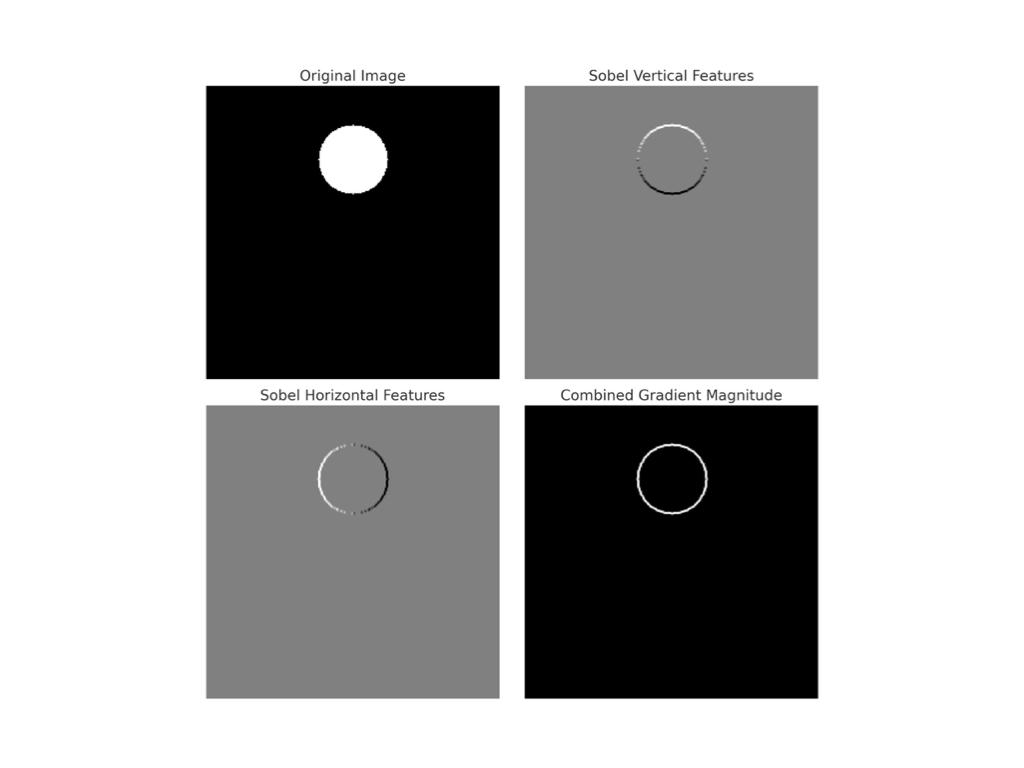
\includegraphics[width=0.7\textwidth]{figure2.jpg}
\caption{Illustration of Sobel Operator in Edge Detection.}
\end{figure}

In this work, the Sobel operator is utilized as a feature extraction method, with the goal of aiding the regression model in identifying essential patterns and improving its predictive performance.

\subsubsection{Fast Fourier Transform (FFT)}
The Fast Fourier Transform (FFT) of an image converts the spatial domain representation of the image into the frequency domain. This transformation represents the image as a combination of sinusoidal waves with varying frequencies and amplitudes. The FFT helps analyze and process the frequency components, such as identifying high-frequency details (edges, noise) or low-frequency patterns (smooth regions). It is widely used in image processing tasks like filtering, compression, and feature extraction, as it enables efficient manipulation and enhancement of image characteristics that are difficult to address in the spatial domain.

\begin{figure}[H]
\centering
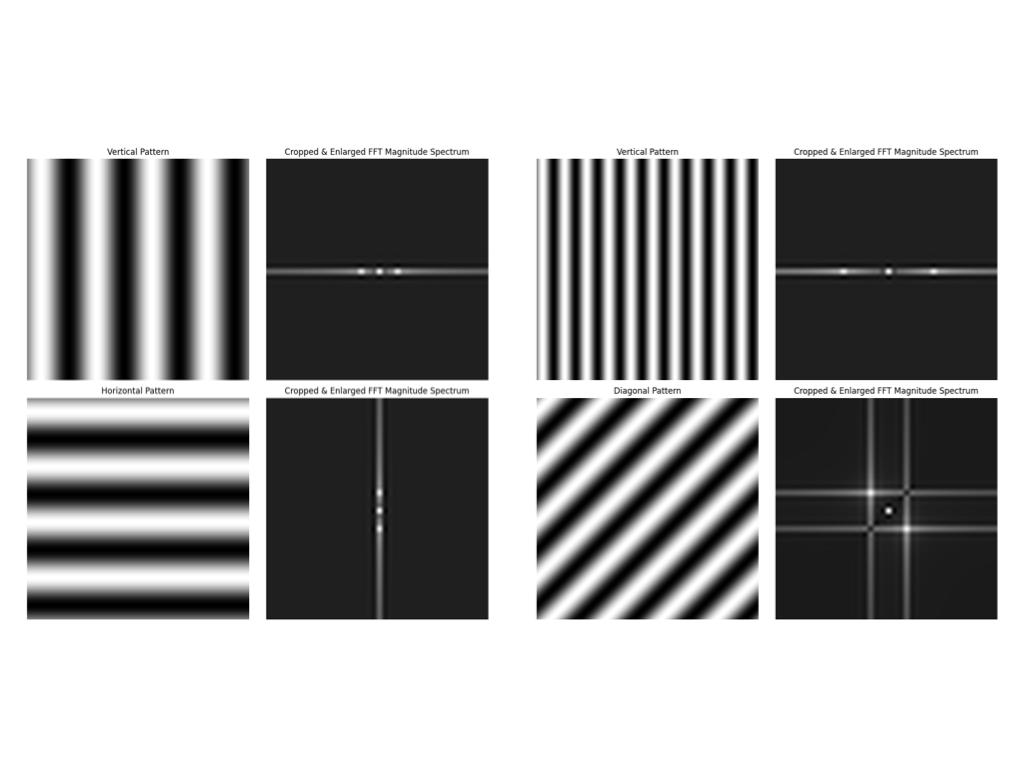
\includegraphics[width=0.6\textwidth]{figure3.jpg}
\caption{FFT illustration: proximity to the center represents low-frequency features, while the outer regions highlight high-frequency details.}
\end{figure}

Compared to spatial-domain features, which are more intuitive for human visual perception, the frequency domain often provides insights into details that may not be easily noticeable to the naked eye. This is particularly evident in cases where the image contains linear motion blur. In such scenarios, the frequency-domain representation clearly highlights patterns and directional features of the blur, enabling precise analysis and identification of the blur’s characteristics.

\begin{figure}[H]
\centering
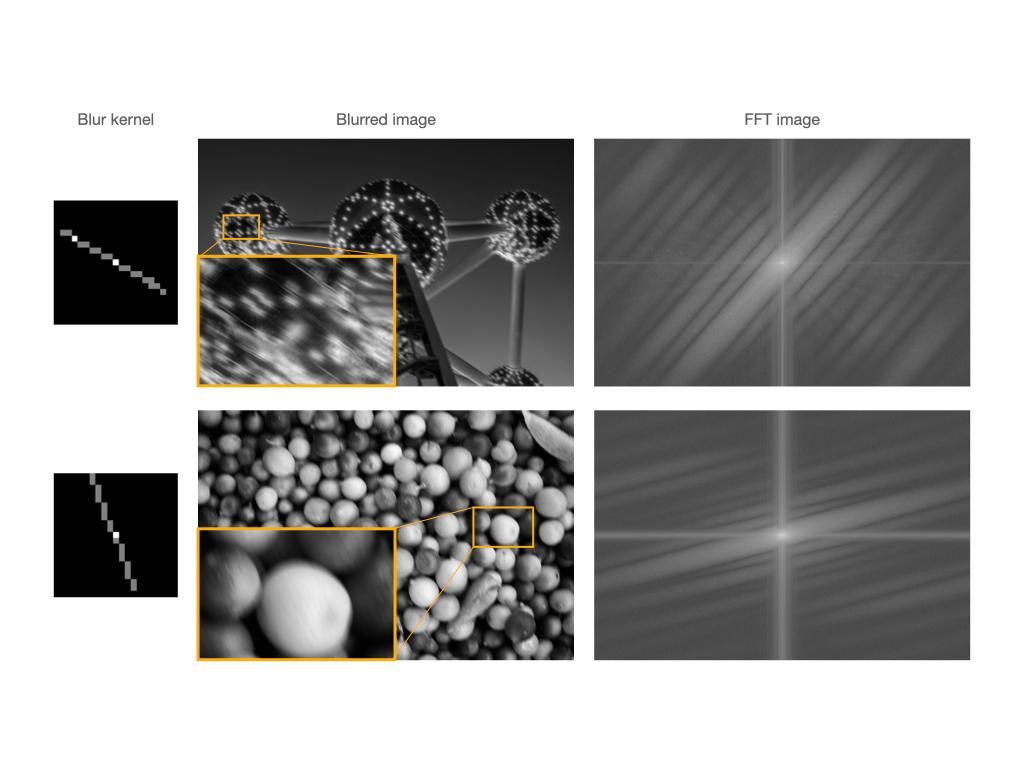
\includegraphics[width=0.6\textwidth]{figure4.jpg}
\caption{Linear Motion FFT Plot. This plot demonstrates the relationship between the blur kernel and the FFT of the blurred image.}
\end{figure}


\section{Methodology}

\subsection{Blur Kernel Settings}
In this research, we focus on two different types of blur: Gaussian blur and motion blur.
Gaussian blur is a type of image blurring that uses a Gaussian function to smooth the image. It is often used to reduce noise or detail, and it also can be used to imitate the defocus of a camera.
The Gaussian blur kernel is derived from the Gaussian function and can be described as:

\subsubsection{Gaussian Blur}
Gaussian blur is modeled using the function:
\[
G(x, y) = \frac{1}{2\pi\sigma^2} \exp\left(-\frac{x^2 + y^2}{2\sigma^2}\right)
\]
 \( (x, y) \) are the coordinates of a point in the kernel (relative to center, and \( \sigma \) is the standard deviation, which controls the spread of the blur (larger  \( \sigma \) means a more blurred image).
As for motion blur, it simulates the effect of a moving camera or object. The blur is directional, and the kernel typically represents a linear motion along a specific angle.

\subsubsection{Motion Blur}
For a motion blur of length  L  along an angle \(\theta\) , the kernel  H(x, y)  can be represented as:
\[
H(x, y) =
\begin{cases}
\frac{1}{L} & \text{if } |x \cos \theta + y \sin \theta| \leq \frac{L}{2}, \\
0 & \text{otherwise}.
\end{cases}
\]

\begin{figure}[H]
\centering
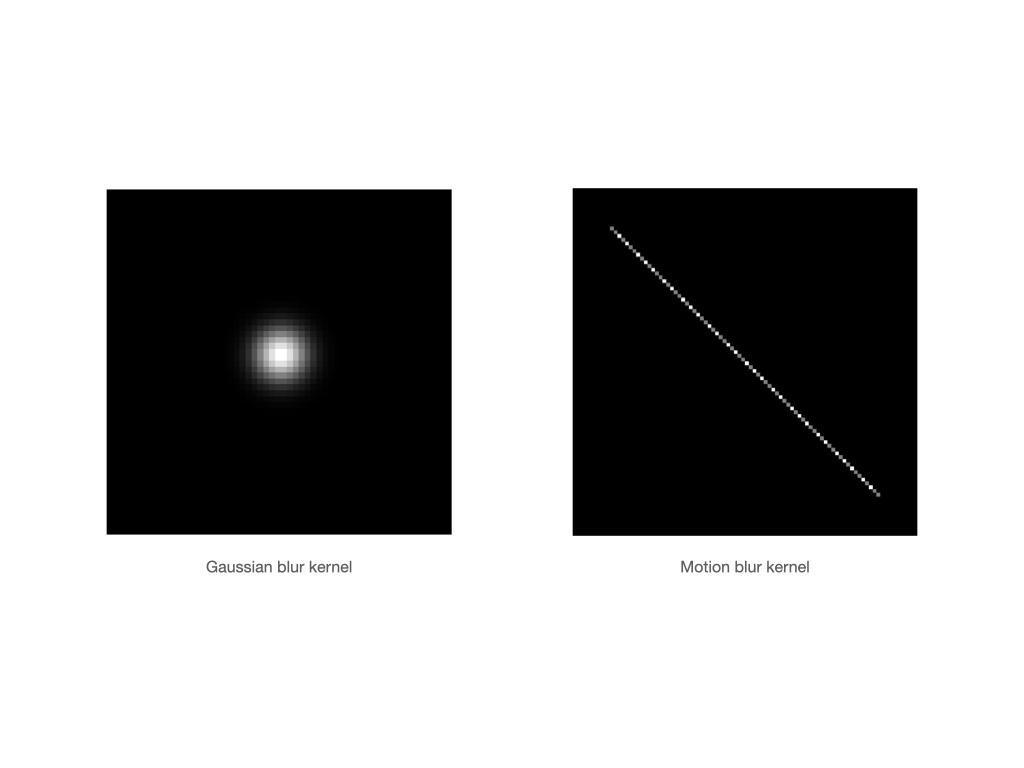
\includegraphics[width=0.6\textwidth]{figure5.jpg}
\caption{Illustration of blur kernel.}
\end{figure}

\subsection{Training Process}
Our training methodology centers on developing an effective pipeline for blur kernel estimation through machine learning. After the initial preprocessing steps, we implement a two-stage feature extraction process that combines spatial and frequency domain information. These are complementary features that help capture both local structural details and also global blur patterns that are essential for accurate kernel prediction.
The regression task is a unique challenge due to the complex relationship between image features and blur characteristics. To address this, we explore two distinct prediction strategies. The first strategy, which we call the parameter-based approach, treats blur estimation as a low-dimensional regression problem. For Gaussian blur, the model predicts only the sigma value, while for motion blur, it estimates the angle of motion. This approach benefits from its simplicity and direct connection to the physical properties of the blur process.
Our second strategy, the direct kernel prediction approach, is a more ambitious goal. Instead of predicting blur parameters, the model attempts to reconstruct the entire 21×21 kernel matrix directly from the extracted features and although this increases the complexity of the regression task, it offers greater flexibility in capturing real-world blur patterns that may deviate from ideal parametric models.

\begin{figure}[H]
\centering
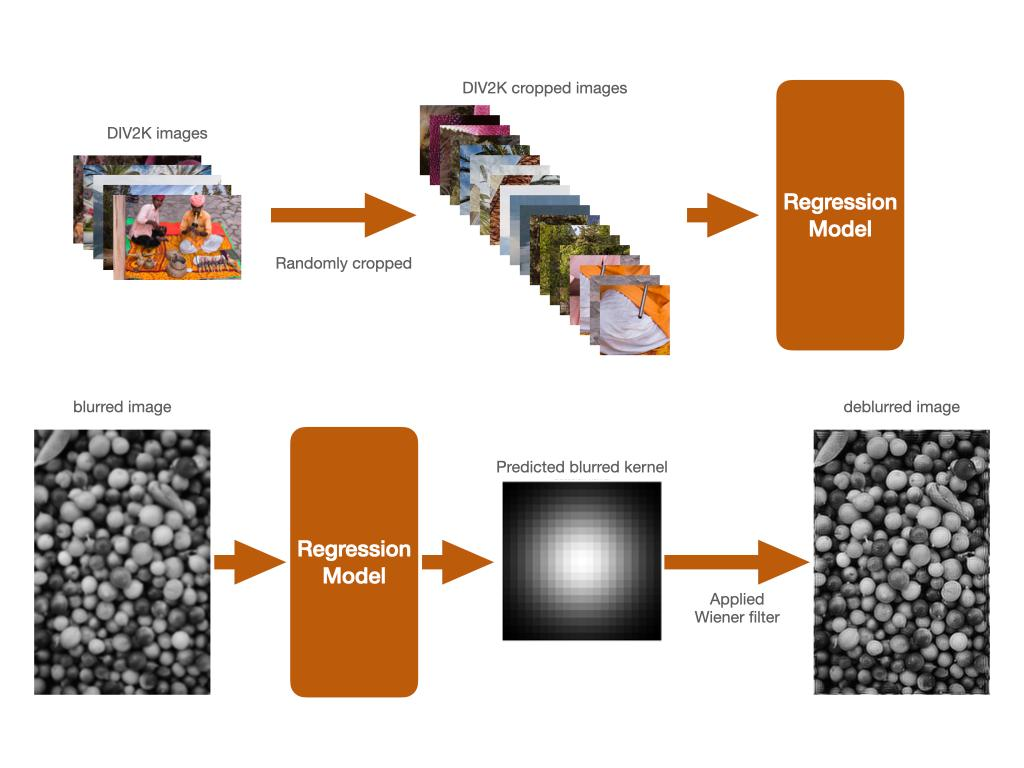
\includegraphics[width=0.65\textwidth]{figure6.jpg}
\caption{Training and Application Flowchart.}
\end{figure}

We apply these strategies using three different regression algorithms, each chosen for its particular strengths. Random Forest Regression, which uses ensemble learning to handle the non-linear relationships between image features and blur patterns. Support Vector Machines with specialized kernels help capture complex mappings in the feature space, while k-Nearest Neighbors provides locally adaptive predictions that can accommodate varying blur characteristics across different image regions.
The testing phase implements an end-to-end pipeline where new images undergo the same feature extraction process before kernel prediction. These predicted kernels then feed into the Wiener filter for final image restoration. This systematic approach lets us check both the accuracy of our kernel predictions and also the effectiveness in practical deblurring applications.

\subsection{Wiener Filter}
The Wiener filter provides a mathematical framework for image restoration, but its effectiveness depends heavily on accurate blur kernel estimation. Traditional approaches to kernel estimation often rely on trial-and-error, making the restoration process time-consuming and potentially unreliable. This limitation motivates our use of machine learning techniques to predict appropriate blur kernels directly from image features. In the frequency domain, the Wiener filter reconstructs an estimate of the original image by applying a carefully designed filter to the blurred input. Working with frequency representations allows us to treat the blur as a multiplication operation rather than a more complex convolution. Let g(x,y) represent our observed blurred image, f(x,y) be the unknown clean image we aim to recover, and h(x,y) denote the blur kernel responsible for the degradation.
The core operation of the Wiener filter in the frequency domain takes the form:

\[
\hat{F}(w) = \frac{H(w)^* \cdot G(w)}{|H(w)|^2 + \text{noise}}
\]
where \(F(w)\) is the Fourier transform of the estimated original image; \(G(w)\) is the Fourier transform of the observed image g(x, y); \(H(w)\) is the Fourier transform of the blur kernel h(x, y); \(H(w)^*\) is the complex conjugate of \(H(w)\); \(|H(w)|^2\) is the squared magnitude of the blur kernel in the frequency domain. The denominator term \(|H(w)|^2\) + noise helps stabilize the restoration process, preventing the amplification of noise in frequencies where the blur kernel has very small values.
The presence of the noise term in the denominator highlights a key practical consideration - there is always a trade-off between blur removal and noise amplification. A larger noise term produces a more conservative restoration that preserves some blur but suppresses noise, while a smaller term attempts more aggressive deblurring at the risk of amplifying noise artifacts. 

\begin{figure}[!ht]
\centering
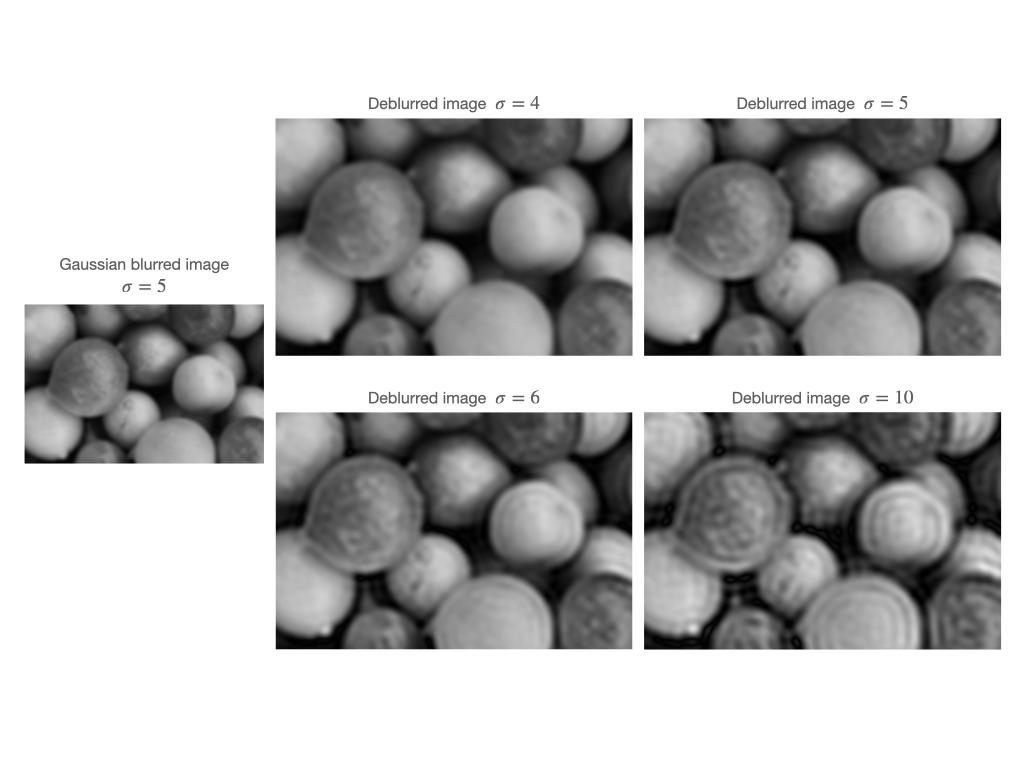
\includegraphics[width=0.4\textwidth]{figure7.jpg}
\caption{Deblurring the image using the Wiener filter with different blur kernels. 
Finding the appropriate blur kernel  h(x, y)  is crucial for effectively restoring a blurred image. Once we identify the correct kernel, we can better recover the original image and reduce the effects of blurring.}
\end{figure}

\FloatBarrier 

\section{Results}
Predicting the sigma value (for Gaussian blur) or the angle (for motion blur) requires understanding details in the image. These features might not be easy to capture with shallow models like Random Forests, especially when the relationship between the image content and the blur parameters is highly nonlinear or complex. (Table \ref{tab:performance}).

\begin{table}[h]
\caption{Performance Metrics for Different Models}
\label{tab:performance}
\begin{center}
\begin{tabular}{lccc}
\hline
Model & MAE\_Global & MSE\_Global & R2\_Global \\
\hline
RF & 0.01264755 & 0.00214398 & 0.7748670 \\
KNN & 0.01264454 & 0.00204710 & 0.7968311 \\
SVM & 0.00933183 & 0.00214543 & 0.7891896 \\
\hline
\end{tabular}
\end{center}
\end{table}

The performance metrics reveal several key insights about the models' capabilities in predicting blur parameters:

The Support Vector Machine (SVM) achieved the lowest Mean Absolute Error (MAE) at $0.00933$, approximately $26\%$ better than both Random Forest and KNN models which had MAE values around $0.0126$. This suggests that SVM's ability to handle nonlinear relationships through kernel transformations provided some advantage in capturing blur patterns.

However, examining Mean Squared Error (MSE) shows a different pattern. KNN achieved the lowest MSE at $0.00205$, while RF and SVM had nearly identical MSE values of $0.00214$. The formula for MSE is:

$$
MSE = \frac{1}{n}\sum_{i=1}^{n}(y_i - \hat{y_i})^2
$$

The lower MSE for KNN indicates it makes fewer extreme prediction errors compared to SVM, despite having a higher MAE. This suggests that while SVM makes more accurate predictions on average, it occasionally produces larger outlier errors.

The $R^2$ scores, calculated as:

$$
R^2 = 1 - \frac{\sum(y_i - \hat{y_i})^2}{\sum(y_i - \bar{y})^2}
$$

range from $0.77$ to $0.80$, indicating that approximately $20\%$ of the variance in blur parameters remains unexplained by these models. KNN achieved the highest $R^2$ at $0.797$, suggesting it captures slightly more of the underlying relationship between image features and blur parameters.


\newpage
\section{Conclusion}

Our experiments in predicting blur parameters yielded disappointing results across all tested models. The Random Forest, KNN, and SVM models achieved poor performance metrics, with the high Mean Absolute Error (MAE) values around 0.01 suggest significant deviations from true blur parameters. For motion blur angle prediction, errors frequently exceeded 15 degrees, making the resulting deblurred images visually unsatisfactory. These results indicate that our feature extraction approach, combining Sobel edges and FFT characteristics, failed to capture the complex relationships between image characteristics and blur parameters. The poor performance may be attributed to:

\begin{enumerate}
  \item Insufficient feature engineering to represent blur patterns
  \item Inherent limitations of shallow models in capturing complex image degradation
  \item Potential overfitting to specific blur patterns in our training data
  \end{enumerate}

Further research should explore deep learning approaches or more sophisticated feature extraction methods to improve blur parameter prediction accuracy. The current results suggest this approach is not viable for practical image deblurring applications.

\FloatBarrier 

\newpage
\bibliography{references}

\end{document}
